%Asservissement par traitement d’image d’une plateforme Hexapode

\section*{Contexte}

La caractérisation du système squelettique humain est une donnée importante pour la mise en place de traitements
dédiés en cas de troubles musculo-squelettiques. Des études sur ce sujet existent en utilisant des modélisations
mécaniques de la colonne vertébrale et des simulations numériques par la méthode des éléments finis
par exemple.

Cependant, la validation de ces modèles nécessite la mise en place d’essais expérimentaux. Un dispositif expérimental
étudié par certaines équipes de recherche est organisé autour d’un Hexapode piloté en position. Ce
dispositif est représenté sur la \autoref{fig:01} Le pilotage de la plateforme supérieure est souvent réalisé en asservissant
directement les positions des différents axes. Ce choix technique permet une réalisation facile de la chaine de
commande mais possède un inconvénient : il entraine un manque de précision en raison de la souplesse des vérins
et des jeux dans les liaisons de l’Hexapode.

\begin{figure}[H]
\centering
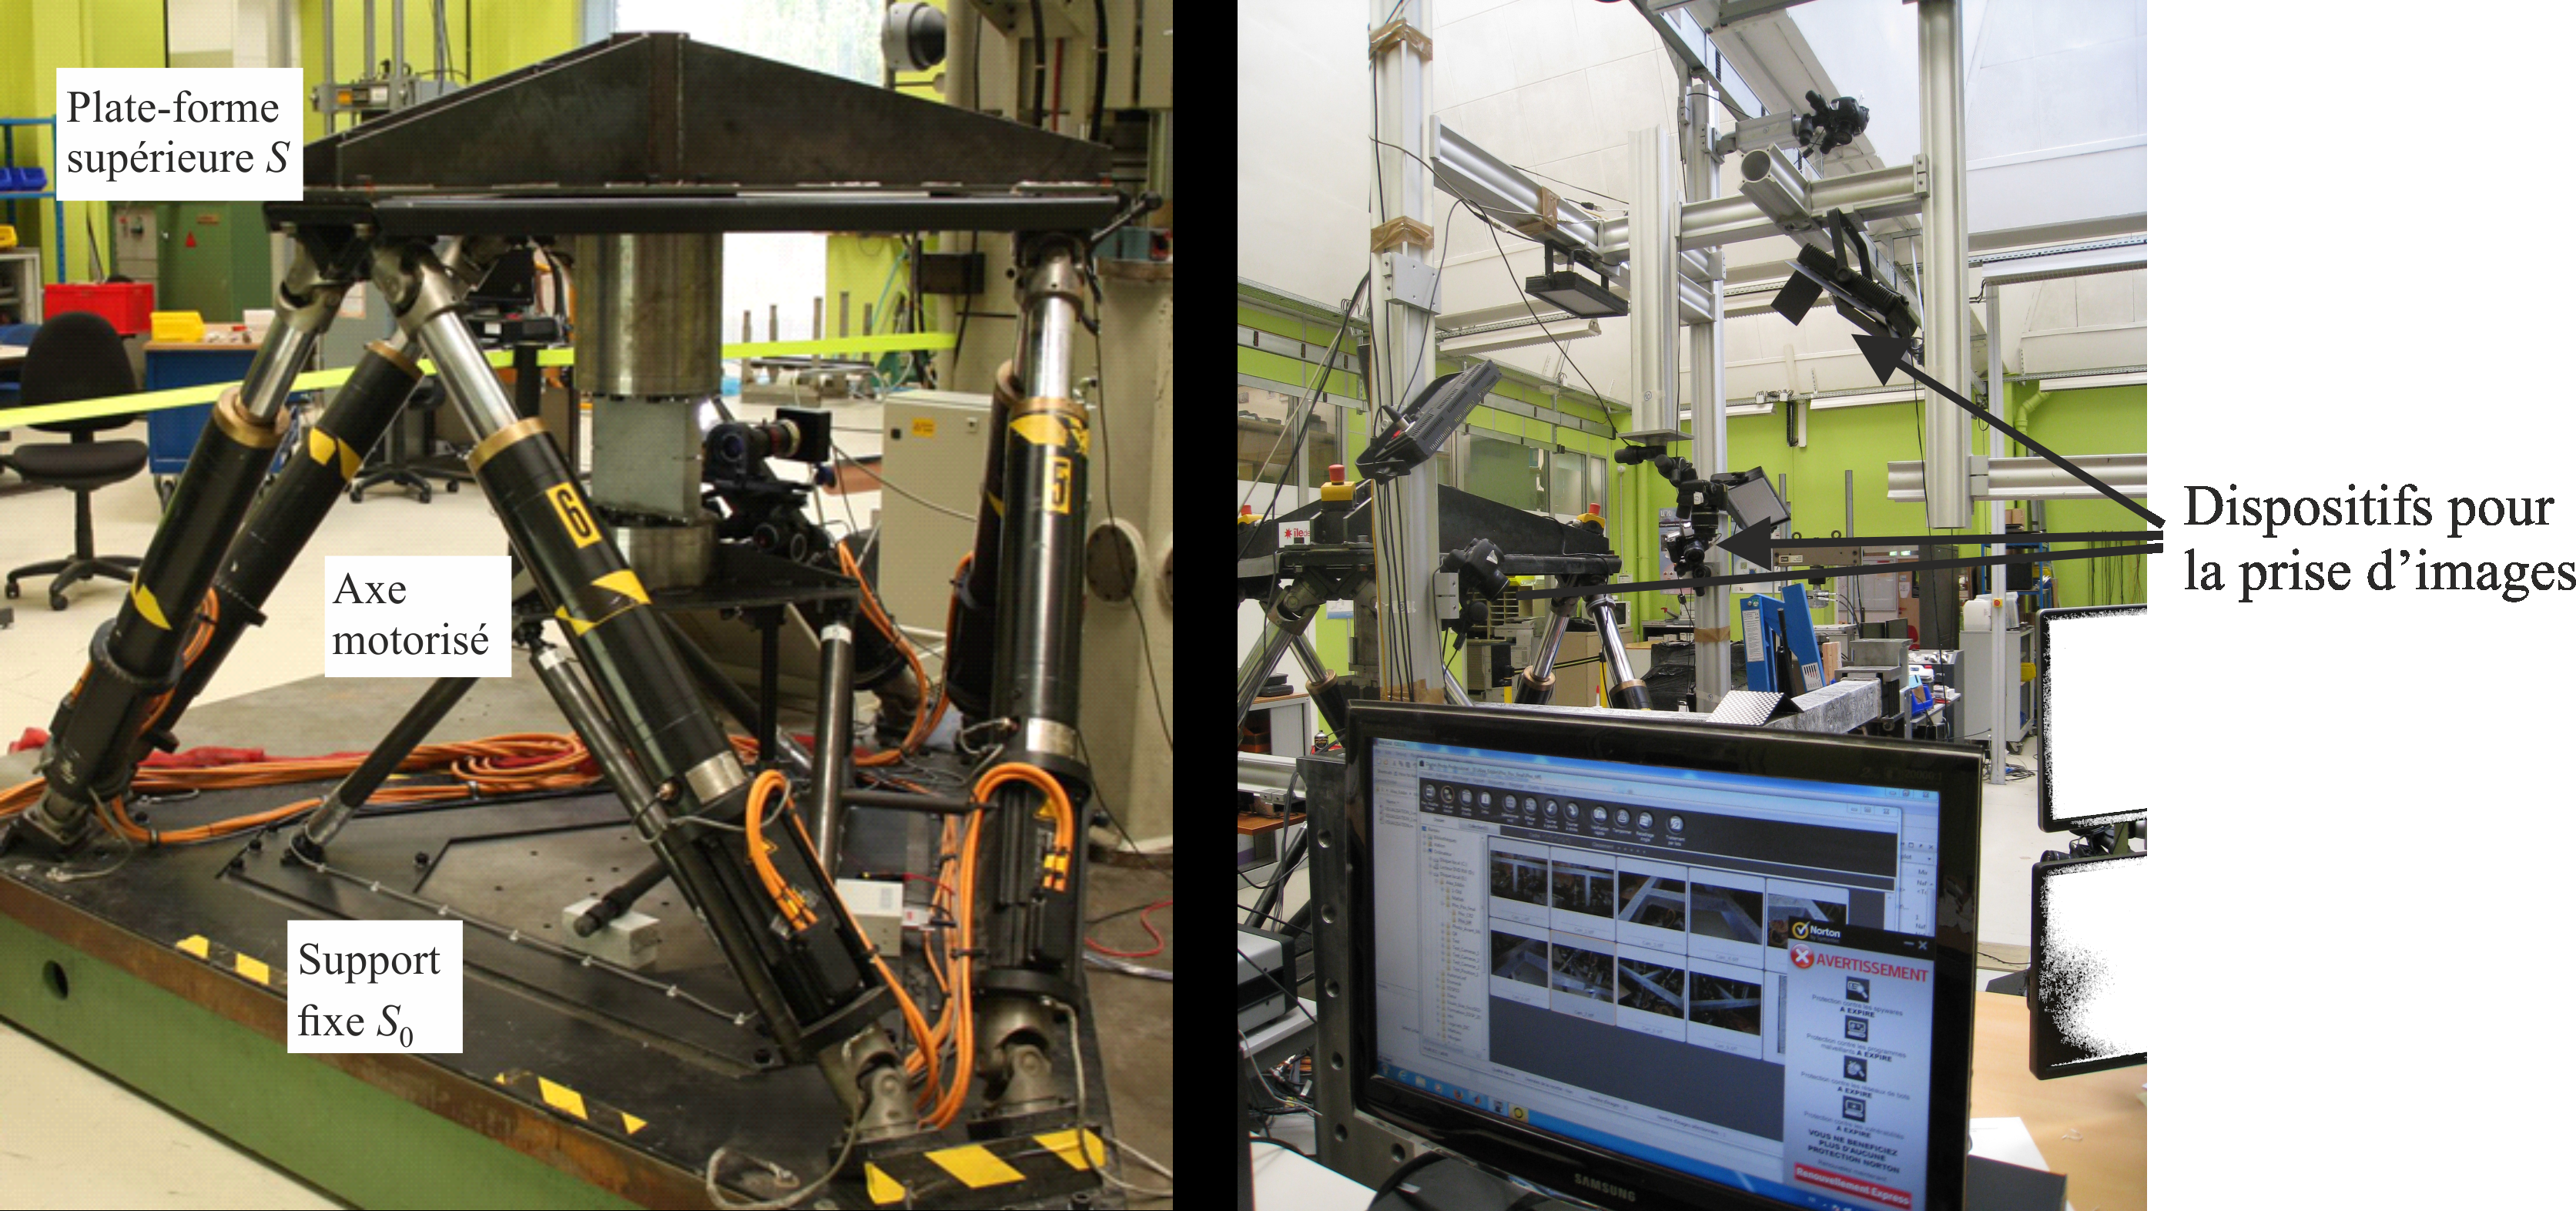
\includegraphics[width=.8\linewidth]{fig_01}
\caption{\label{fig:01} Système d’asservissement en position d’un Hexapode par traitement d’images}
\end{figure}



L’architecture de commande de l’Hexapode est représentée par le schéma de la figure 2. Une des solutions
consiste à asservir les longueurs des vérins $L_i$ à des longueurs de référence $L_i^*$ 
obtenues en utilisant un modèle cinématique inverse à partir des positions souhaitées $P_i^*$ 
de la plateforme dans un repère absolu. Une solution
simple pour déterminer les longueurs des vérins est d’utiliser des mesures issues de capteurs montés directement
sur les axes des moteurs (en tenant compte du rapport de transmission). Mais la simplicité de cette solution
peut conduire à des erreurs en raison de la souplesse des tiges du vérin, ou encore des jeux dans les liaisons,
conduisant ainsi à une longueur de vérin $L_i^d$ 
différente de celle mesurée $L_i^m$. Dans ce contexte, la \autoref{fig:02} propose
deux solutions possibles :
\begin{itemize}
\item la première solution utilise une loi de commande exploitant les seules mesures $L_i^m$ issues des capteurs montés
sur les vérins et entachées d’erreurs dues à la souplesse des tiges et aux jeux éventuels ;
\item une deuxième solution, plus évoluée, exploite une estimation des positions réelles $L_i^{de}$ des extrémités des tiges
des vérins. Une méthode permettant d’obtenir cette estimation est d’utiliser une caméra et un algorithme
de traitement d’images.
\end{itemize}
L’objet de ce sujet est d’évaluer ces solutions et de déterminer une loi de commande permettant d’obtenir
un positionnement de la plateforme selon le cahier des charges représenté sur la figure 3 sous la forme d’un
diagramme des exigences. Ce sujet est décomposé en trois parties :
\begin{itemize}
\item dans la \autoref{sec:01}, il s’agira de développer un modèle mécanique (cinématique) de l’axe ;
\item dans la \autoref{sec:02}, une étude de la précision des axes motorisés sera réalisée en utilisant le modèle développé
dans la \autoref{sec:01} ;
\item enfin dans la \autoref{sec:03}, il s’agira de définir les éléments de l’algorithme de traitement d’images permettant
d’estimer les longueurs réelles des tiges du vérin et de développer des lois de commande permettant d’asservir
la position de la plateforme à une position de référence associée à l’essai à réaliser.
\end{itemize}


\begin{figure}[H]
\centering
\includegraphics[width=.8\linewidth]{fig_02}
\caption{\label{fig:02} Architecture de commande de l’Hexapode }
\end{figure}


\begin{figure}[H]
\centering
\includegraphics[width=.8\linewidth]{fig_03}
\caption{\label{fig:03} Diagramme des exigences }
\end{figure}



\section{\label{sec:01} Étude cinématique de la plateforme Hexapode}

\begin{obj}
Le but de cette partie est d’étudier les mouvements de la plateforme Hexapode afin de définir le modèle
cinématique inverse permettant de déterminer la longueur à imposer aux axes motorisés pour vérifier
un positionnement donné de la plateforme mobile.
\end{obj}
La plateforme Hexapode utilisée ici est constituée des composants suivants, représentés sur les \autoref{fig:04} et \autoref{fig:05} :
\begin{itemize}
\item un support $S_0$, de forme triangulaire, parfaitement lié au sol, et que l’on assimilera au bâti ;
\item une plateforme mobile $S$, de forme triangulaire, dont la mise en position permettra de solliciter expérimentalement
la colonne vertébrale dont l’une des extrémités lui est fixée rigidement ;
\item six axes rectilignes motorisés dont la longueur peut être pilotée, et reliés au niveau de leurs extrémités par
des liaisons sphériques au support $S_0$ d’un côté, à la plateforme $S$ de l’autre.
\end{itemize}

\subsection{ Mouvement d’un axe motorisé (seul) par rapport au support}



\begin{obj}
L’objectif de cette sous-partie est de déterminer les degrés de liberté d’un axe motorisé (seul) par
rapport au support.
\end{obj}

Chaque axe motorisé présente l’architecture illustrée sur la \autoref{fig:04} :
\begin{itemize}
\item un ensemble \{support moteur (13) + corps de vérin (10)\}, relié au support fixe par l’intermédiaire d’une
liaison que l’on peut modéliser par une liaison sphérique (rotule inférieure (14)) ;
\item un ensemble \{actionneur électrique (1) + réducteur (2)\}, fixé au corps de vérin (10) et entrainant la vis (4)
en rotation autour de son axe ;
\item un écrou (5) en liaison par rapport au corps de vérin (10) modélisable par une liaison glissière et en liaison
hélicoïdale par rapport à la vis (4) ;
\item une tige de vérin (7), solidaire de l’écrou (5), et reliée à son extrémité avec la plateforme mobile par l’intermédiaire
d’une liaison que l’on peut modéliser comme une liaison sphérique (rotule supérieure (8)).
\end{itemize}



\begin{figure}[H]
\centering
\includegraphics[width=.8\linewidth]{fig_04}
\caption{\label{fig:04}  }
\end{figure}


%Q01
\question{\label{q:01}À l’aide des informations précédentes, compléter sur le document réponse (figure A) le schéma cinématique
(plan) d’un axe motorisé, en repérant, à l’aide de plusieurs couleurs, l’ensemble \{corps de vérin (10) +
support moteur (13)\}, l’ensemble \{tige de vérin (7) + ecrou (5)\} et la vis (4). On ne tiendra pas compte du
système \{roue (12) + vis sans fin (3)\} associé au capteur (11).}
\ifprof
\begin{corrige}
\end{corrige}
\else
\fi


%Q02
\question{\label{q:02}Déterminer par une méthode à choisir la liaison cinématiquement équivalente à l’ensemble des trois
liaisons présentes entre la tige de vérin (7) et le corps de vérin (10). Représenter sur le document réponse le
schéma cinématique du nouveau modèle (avec la liaison équivalente).}
\ifprof
\begin{corrige}

\end{corrige}
\else
\fi


%Q03
\question{\label{q:03}Déterminer l’expression littérale du vecteur vitesse $\vectv{A}{7}{S_0}$ dans la base $\base{x_1}{y_1}{z_1}$. Combien de
paramètres de mouvement sont alors nécessaires et suffisants pour positionner le point $A$ (centre de la rotule
supérieure (8)) par rapport à $S_0$ ?}
\ifprof
\begin{corrige}

\end{corrige}
\else
\fi



\subsection{Mouvement de la plateforme $S$ par rapport au support $S_0$}

\begin{obj}
L’objectif de cette sous-partie est d’étudier le mouvement de la plateforme en vue de la réalisation
d’un essai spécifique.
\end{obj}


L’architecture de la plateforme Hexapode est représentée sur la \autoref{fig:05} :
\begin{itemize}	
\item au support fixe $S_0$ est attaché le référentiel $\rep{0}\repere{O}{x_0}{y_0}{z_0}$ supposé galiléen, où $\left(O,\vect{x_0},\vect{y_0}\right)$ est le plan
contenant les points $D$, $E$ et $F$;
\item à la plateforme mobile $S$ est attaché le référentiel $\rep{}\repere{G}{x}{y}{z}$ , où $\left(G,\vect{x},\vect{y}\right)$ est le plan contenant les points
$A$,$B$ et $C$;
\item chaque axe $i$ ($1\leq i \leq 6$), relie un point de la plateforme $S$ à un point du support $S_0$ : $\vect{DA}=L_1\vect{u_1}$,
$\vect{DB}=L_2\vect{u_2}$, 
$\vect{EB}=L_3\vect{u_3}$,
$\vect{EC}=L_4\vect{u_4}$,
$\vect{FC}=L_5\vect{u_5}$ et
$\vect{FA}=L_6\vect{u_6}$ où les vecteurs $\vect{u_i}$ sont unitaires.
\end{itemize}

\begin{figure}[H]
\centering
\includegraphics[width=.4\linewidth]{fig_05}
\caption{\label{fig:05} Architecture de la plateforme Hexapode (les liaisons équivalentes
entre tiges et corps de vérins ne sont pas représentées). }
\end{figure}

%Q04
\question{\label{q:04} À l’aide du nombre de paramètres de mouvement (déterminé à la question \ref{q:03}) du centre de la rotule
supérieure de chaque axe motorisé et du nombre de relations scalaires indépendantes que l’on peut écrire à
propos des positions de ces centres, montrer que la plateforme mobile $S$ a six degrés de liberté par rapport au
support $S_0$.}
\ifprof
\begin{corrige}
\end{corrige}
\else
\fi

Dans la suite, on choisira comme degrés de liberté les trois coordonnées cartésiennes de la position du centre de
gravité $G\left(x_G,y_G,z_G\right)_{\rep{0}}$ de la plateforme mobile $S$ dans $\rep{0}$, ainsi que les trois angles d’Euler $\left(\psi, \theta, \phi\right)$ définis
dans la \autoref{fig:06}.

Afin de pouvoir solliciter la colonne vertébrale testée, la plateforme mobile $S$ doit pouvoir être pilotée de façon à
ce que le triangle ABC soit contenu dans un plan ($\Pi$) dont l’équation cartésienne dans $\rep{0}$ est ($\Pi$) : $z=ax+by+c$
où $\left(x,y,z\right)$ sont les coordonnées dans $\rep{0}$ d’un point $M$ de ($\Pi$) et $(a,b,c)$ sont trois constantes non nulles.

\begin{figure}[H]
\centering
\includegraphics[width=.8\linewidth]{fig_06}
\caption{\label{fig:06} Définition des trois angles d’Euler (précession $\psi$, nutation $\theta$, rotation propre $\phi$).}
\end{figure}


%Q05
\question{\label{q:05} Déterminer l’équation cartésienne dans $\rep{0}$ du plan de la plateforme mobile $S$ à l’aide des six degrés
de liberté $\left( x_G,y_G,z_G, \psi, \theta, \phi \right)$ de cette dernière. Pour cela, on calculera le produit scalaire 
$\vect{GM}\cdot \vect{n}$, où $\vect{n}$ est le
vecteur normal unitaire à la plateforme mobile que l’on exprimera à l’aide des vecteurs de la base $\base{x}{y}{z}$. En
déduire qu’il est possible de relier les degrés de liberté $\left( x_G,y_G,z_G, \psi, \theta\right)$ de la plateforme mobile $S$ aux constantes
$\left(a,b,c\right)$ de l’équation cartésienne de ($\Pi$) ; on ne cherchera pas à expliciter les fonctions donnant l’expression de
$\left( x_G,y_G,z_G, \psi, \theta\right)$ en fonction de $\left(a,b,c\right)$. Pourquoi l’angle de rotation propre $\phi$ n’intervient-il pas dans l’équation
demandée ?}
\ifprof
\begin{corrige}
\end{corrige}
\else
\fi


Ces relations permettent de déterminer les valeurs des degrés de liberté de la plateforme mobile $S$ pour lesquels
cette dernière se positionne dans le plan ($\Pi$), caractérisant ainsi l’essai effectué sur la colonne vertébrale. Pour
fixer ces degrés de liberté, il faut déterminer quelles consignes de longueurs doivent être appliquées aux six
vérins de la plateforme mobile.
Les trois sommets du support fixe $S_0$ vérifient les relations suivantes :
\begin{itemize}
\item $\vect{OD}=-\dfrac{\sqrt{3}R}{2}\vect{x_0}+\dfrac{R}{2}\vect{y_0}$;
\item $\vect{OE}=-R\vect{y_0}$;
\item $\vect{OF}=\dfrac{\sqrt{3}R}{2}\vect{x_0}+\dfrac{R}{2}\vect{y_0}$.
\end{itemize}

Les trois sommets de la plateforme mbil $S_0$ vérifient les relations suivantes :
\begin{itemize}
\item $\vect{GA}=R\vect{y}$;
\item $\vect{GB}=-\dfrac{\sqrt{3}R}{2}\vect{x}-\dfrac{R}{2}\vect{y}$;
\item $\vect{GC}=\dfrac{\sqrt{3}R}{2}\vect{x}-\dfrac{R}{2}\vect{y}$.
\end{itemize}


On supposera dans toute la suite de cette étude que $x_G = y_G = 0$ et $\phi=0$.

%Q6
\question{\label{q:06} Déterminer littéralement la longueur $L_1 = D1$ de l’axe motorisé 1, en fonction de $\left(z_G,\psi,\theta\right)$.
Les autres longueurs de vérins peuvent être déterminées de façon analogue. L’ensemble des relations obtenues
constitue ce que l’on appelle le modèle de cinématique inverse de la plateforme Hexapode, dont la connaissance
est nécessaire pour élaborer la commande en position de la plateforme mobile $S$ en vue de la réalisation de
l’essai sur la colonne vertébrale.}
\ifprof
\begin{corrige}
\end{corrige}
\else
\fi


%Q07
\question{\label{q:07} Donner les expressions littérales des degrés de liberté  $\left( x_G,y_G,z_G, \psi, \theta, \phi \right)$ de la plateforme mobile $S$
lorsque l’on impose que la longueur de chaque axe motorisé $i$ est identique ($L_i = L, \forall i$). On pourra recourir à des arguments de symétrie pour justifier ce positionnement. Sachant que $R=\SI{0,65}{m}$, faire les applications numériques pour $L=L_{\text{min}}=\SI{0,75}{m}$
et $L=L_{\text{max}}=\SI{1,5}{m}$; en déduire l’amplitude du mouvement de translation
verticale de la plateforme mobile $S$. Vérifier si l’exigence correspondante du cahier des charges, donné \autoref{fig:03},
est validée.}
\ifprof
\begin{corrige}
\end{corrige}
\else
\fi

\section{Précision en position de la plateforme mobile}
\begin{obj}
Le but de cette partie est de proposer un modèle d’axe motorisé permettant de quantifier les phénomènes qui dégradent la précision en position de la plateforme mobile
\end{obj}

On rappelle que l’architecture d’un axe motorisé est détaillée sur la \autoref{fig_04}. On y voit notamment que la mesure
de la position angulaire de l’axe de l’actionneur électrique (1) se fait grâce à une roue codée (11), entrainée
par l’intermédiaire d’un dispositif \{roue (12) + vis sans fin (3)\} dont la vis est montée sur l’arbre de sortie du
réducteur (2) ; le rapport de transmission associé est $\dfrac{\omega_{12}}{\omega_{3}}= \dfrac{1}{10}$.


%Q08
\question{\label{q:08} Étant donné que l’information de la roue (12) est codée sur 15 bits et que le pas (par tour) de la liaison
hélicoïdale \{vis (4) + écrou (5)\} est de \SI{5}{mm}, quelle est la résolution théorique en translation d’un axe motorisé ?
Comparer avec les exigences de la \autoref{fig_03}.}
\ifprof
\begin{corrige}
\end{corrige}
\else
\fi

\subsection{Détermination des efforts sur les axes motorisés}
\begin{obj}
L’objectif de cette sous-partie est de déterminer, pour une position donnée de la plateforme mobile, les
efforts appliqués sur les différents axes motorisés, qui auront une influence sur la précision en position
de ces derniers.
\end{obj}


Les différents éléments de la plateforme Hexapode sont soumis aux actions mécaniques suivantes :
\begin{itemize}
\item l’action de la colonne vertébrale testée sur la plateforme mobile $S$ est modélisée par 
$\torseurstat{T}{\text{colonne vertébrale}}{S} = 
\torseurl{\vect{F}=F_X\vect{x_0}+F_Y\vect{y_0}+F_Z\vect{z_0}}
{\vect{C}=C_X\vect{x_0}+C_Y\vect{y_0}+C_Z\vect{z_0}}{G}$;
\item l’action de la pesanteur sur la plateforme mobile $S$ est modélisée par 
$\torseurstat{T}{\text{pesanteur}}{S} = \torseurl{\vect{P}=-mg\vect{z_0}}{\vect{0}}{G}$;
\item l'action de la plateforme mobile $S$ sur un axe $i$, transmise par la liaison sphérique correspondante (supposée parfaite), est modélisée par
$\torseurstat{T}{S}{\text{axe } i} = \torseurl{\vect{F_i}}{\vect{0}}{\text{centre de la liaison sphérique}}$;
\item l'action de la plateforme mobile $S_0$ sur un axe $i$, transmise par la liaison sphérique correspondante (supposée parfaite), est modélisée par
$\torseurstat{T}{S_0}{\text{axe } i} = \torseurl{\vect{F_i^0}}{\vect{0}}{\text{centre de la liaison sphérique}}$;
\end{itemize}

On négligera la masse des différents constituants des axes motorisés, et on supposera que les mouvements de la
plateforme Hexapode sont suffisamment lents pour que l’on puisse négliger dans les équations tous les termes
d’inertie.

%Q09
\question{\label{q:09} On considère ici l’axe motorisé 1, qui est tel que $\vect{DA}=L_1(t) \vect{u_1}(t)$. En isolant l’ensemble de ses pièces constitutives, situées entre la rotule supérieure (8) (de centre $A$) et la rotule inférieure (14) (de centre $D$), déterminer la direction des résultantes $\vect{F}$ et  $\vect{F_1^0}$ des actions de liaison sur l’axe motorisé 1.}
\ifprof
\begin{corrige}
\end{corrige}
\else
\fi


%Q
\question{\label{q:10} Montrer que les intensités $F_i$ des résultantes $\vect{F_i}$ ($1\leq i \leq 6$) vérifient le système matriciel suivant :}
$$
\begin{pmatrix}
M_{11} & ... & M_{16} \\
\vdots    &     & \vdots \\
M_{61} & ... & M_{66} \\
\end{pmatrix}
\begin{pmatrix}
F_1 \\ F_2 \\ F_3 \\ F_4 \\ F_5 \\ F_6 \\
\end{pmatrix}
=
\begin{pmatrix}
F_X \\ F_Y \\ F_Z-mg \\ C_X \\ C_Y \\ C_Z \\
\end{pmatrix}
$$
\textit{où les composantes $M_{ij}$ de la matrice $M$ de dimension $6\times 6$ sont des fonctions scalaires des degrés de liberté
de la plateforme mobile $S$; on donnera notamment l’expression des termes $M_{k1,1\leq k \leq 6}$ de la première colonne
de $M$ sous la forme de produits scalaires et de produits mixtes que l’on ne cherchera pas à développer.}
\ifprof
\begin{corrige}
\end{corrige}
\else
\fi


%Q11
\question{\label{q:11}En adoptant pour chaque axe le modèle de liaison équivalente déterminé dans la question \ref{q:02}, montrer,
par une méthode à choisir, qu’il est possible de déterminer l’ensemble des efforts de liaison agissant dans une
position donnée de la plateforme mobile $S$, et par conséquent, que la matrice $M$ est inversible.
On obtient ainsi, pour une position donnée de la plateforme mobile $S$, et un chargement fixé sur la colonne
vertébrale, les efforts subis par chaque axe motorisé. Ces efforts seront utilisés dans la suite pour estimer la
précision en position d’un axe motorisé.}
\ifprof
\begin{corrige}
\end{corrige}
\else
\fi

\subsection{Prise en compte de la rigidité du dispositif vis-écrou}
\begin{obj}
L’objectif de cette sous-partie est de prendre en compte les imperfections du système vis-écrou qui
affectent la précision en position d’un axe motorisé, et de quantifier cette dernière.
\end{obj}

La liaison hélicoïdale est réalisée par un dispositif vis-écrou à billes avec un écrou précontraint. On estime que
la source majeure d’imprécision dans le positionnement d’un axe motorisé provient de la rigidité globale de
ce dispositif qui est soumis à une charge axiale $F_a$ : plus cette rigidité est élevée, meilleure est la précision
en position d’un axe motorisé. Afin de modéliser cette rigidité globale, on suppose que le comportement de
déformation axiale de chacun des constituants peut être modélisé par un ressort de traction-compression
\begin{itemize}
\item un ressort de raideur $K_e$ pour modéliser la déformation axiale de l’écrou provoquée par la charge axiale
$F_a$ : $F_a = K_e \Delta L_e$,  où $\Delta L_e$ est la variation de longueur axiale de l’écrou ;
\item un ressort de raideur $K_v$ pour modéliser la déformation axiale de la vis provoquée par la charge axiale $F_a$ : $F_v = K_v \Delta L_v$,  où $\Delta L_v$ est la variation de longueur axiale de la vis ;
\item n ressort de raideur $K_b$ pour modéliser la déformation axiale de l’ensemble des billes en contact, provoquée par la charge axiale $F_a$ : $F_a = K_b \Delta L_b$,  où $\Delta L_b$ est la variation de longueur axiale des billes.
\end{itemize}

%Q12
\question{\label{q:12}Donner l’expression littérale de la rigidité globale $K_g$ de l’ensemble \{vis -- écrou\}, définie comme le quotient de la charge axiale $F_a$  appliquée à l’ensemble et de la variation de longueur axiale $\Delta L_a = \Delta L_e + \Delta L_v + \Delta L_b$ de l’ensemble.}
\ifprof
\begin{corrige}
\end{corrige}
\else
\fi

La \autoref{fig:07} représente les courbes caractéristiques \{charge -- déplacement\} du dispositif vis-écrou selon que l’écrou utilisé est précontraint ou non ; à l’aide de celles-ci, il est en particulier possible d’estimer, pour une
valeur donnée de la charge axiale $F_a$, la raideur $K_b$ définie plus haut comme la pente de la tangente à la courbe considérée au point correspondant à la charge $F_a$.


\begin{figure}[H]
\centering
\includegraphics[width=.6\linewidth]{fig_07}
\caption{\label{fig:07}  Courbe \{charge axiale -- déplacement axial\} d’un dispositif vis-écrou liée à la
déformation des billes.}
\end{figure}


%Q13
\question{\label{q:13}À l’aide de la \autoref{fig:07}, expliquer pourquoi il est plus avantageux d’utiliser un écrou précontraint pour améliorer la précision en position d’un axe motorisé.}
\ifprof
\begin{corrige}
\end{corrige}
\else
\fi


On cherche maintenant à estimer l’erreur de positionnement de la plateforme $S$ dans une situation donnée :
\begin{itemize}
\item la longueur de chaque axe motorisé est égale à $L$;
\item chaque axe motorisé subit une charge axiale de compression $\vect{F}_i=F_a \vect{u_i}$ avec $F_a = \SI{1}{kN}$.
\end{itemize}

Dans cette situation, les raideurs $K_e$ et $K_b$ sont constantes et identiques pour les six axes, tandis que la raideur associée à la vis seule peut s’exprimer comme $K_v = \dfrac{E_v A_v}{L_v}$ où :
\begin{itemize}
\item $E_v$ est le module de Young qui caractérise la rigidité du matériau constitutif de la vis ;
\item $A_v$ est l’aire de la section de la vis ;
\item $L_v$ est la longueur de vis sollicitée en compression, qui varie selon la position de l’écrou de $\indice{L}{v min}= \SI{0}{mm}$ (quand la tige du vérin est complètement rentrée) à $\indice{L}{v max}= \SI{750}{mm}$ (quand la tige du vérin est complètement
sortie).
\end{itemize}

%Q14
\question{\label{q:14} Donner l’expression littérale, puis numérique (en unités SI) des valeurs maximale et minimale de la raideur $K_g$. On utilisera pour cela : $K_e = \SI{734}{N.\mu m^{-1}}$, 
$K_b = \SI{970}{N.\mu m^{-1}}$, $E_v = \SI{210}{GPa}$
 et $A_v = \SI{3200}{mm^2}$.} 
\ifprof
\begin{corrige}
\end{corrige}
\else
\fi


%Q15
\question{\label{q:15} Dans les cas successifs d’un vérin entièrement rentré ($L_v = L_{v\text{ min}}=\SI{0}{mm}$) et d’un vérin entièrement
sorti ($L_v = L_{v\text{ max}}=\SI{750}{mm}$), calculer la variation de longueur de l’axe motorisé due à la charge de compression axiale $-F_a$. Comparer ces variations avec la résolution théorique d’un axe motorisé, déterminée à la question \ref{q:08}.
Conclure vis-à-vis du diagramme des exigences de la \autoref{fig:03}.}
\ifprof
\begin{corrige}
\end{corrige}
\else
\fi


%Q16
\question{\label{q:16}Déduire de la question précédente l’écart de positionnement maximal 
 $\left(\Delta x_G, \Delta y_G, \Delta z_G, \Delta\psi, \Delta\theta, \Delta\phi\right)$, dû
à la rigidité globale des dispositifs \{vis -- écrou\}, de la plateforme mobile $S$ lorsque celle-ci est dans les deux
positions définies à la question \ref{q:07}. Conclure vis-à-vis du diagramme des exigences de la \autoref{fig:03}.}
\ifprof
\begin{corrige}
\end{corrige}
\else
\fi

\section{\label{sec:03} Asservissement par traitement d’images}
\begin{obj}
L’objectif de cette partie est d’une part de définir une mesure du positionnement de la plateforme
mobile à l’aide d’un algorithme de traitement d’images, et d’autre part de concevoir une loi de commande permettant d’asservir la position de la colonne vertébrale, liée à la plateforme, à une position
de référence.
\end{obj}

\subsection{Construction de l’algorithme d’estimation par traitement d’images}

\begin{obj}
L’objet de cette sous-partie est la construction d’un algorithme permettant d’obtenir la position de la
colonne vertébrale exprimée dans un repère absolu.
\end{obj}

Le positionnement de la plateforme mobile est déterminé à l’aide d’images fixes capturées par plusieurs caméras
placées autour de la plateforme Hexapode (voir \autoref{fig:01}). Par souci de simplification, on ne s’intéressera dans
la suite qu’au traitement des images d’une seule de ces caméras.
Une image peut être représentée sous la forme d’un tableau de valeurs, chaque case correspondant à un pixel de
l’image ; les caméras étant monochromatiques, chaque valeur du tableau représente le niveau de gris codé sur 8
bits du pixel correspondant (pour information : $0=$noir, $255=$blanc). Pour simplifier le problème, on admet que
chaque image peut être représentée par une fonction continue des variables continues de l’espace 2D :
\begin{itemize}
\item $f(X,Y)$ désigne l’image de référence, associée à la plateforme en position nominale supposée connue (comme
illustré à titre d’exemple sur la \autoref{fig:08}) ;
\item $g(X,Y)$ désigne une image prise à un instant donné (voir \autoref{fig:08}) ;
où $X$ et $Y$ désignent respectivement l’abscisse et l’ordonnée d’un point $M$ de l’image (voir \autoref{fig:09}).
\end{itemize}


\begin{figure}[H]
\centering
\includegraphics[width=\linewidth]{fig_08}
\caption{\label{fig:08}  Images en position nominale et décalée}
\end{figure}


\begin{figure}[H]
\centering
\includegraphics[width=.4\linewidth]{fig_09}
\caption{\label{fig:09}  Repère image}
\end{figure}

L’objet de l’algorithme de traitement d’images est de trouver le déplacement $\vect{U}(X,Y)$, de composantes $U_X(X,Y)$ et 
$U_Y(X,Y)$ dans le repère de l’image, qui permet de relier l’image de référence à l’image actuelle :
$$g\left( X + U_X(X,Y),Y + U_Y(X,Y)\right) = f(X,Y)+n(X,Y)$$
où $n(X,Y)$ désigne un « bruit de mesure » (ce terme modélise, entre autres, des erreurs dans la prise d’images et
dans la discrétisation des signaux). Le principe de l’algorithme est de minimiser la fonction « cout » suivante 
$$J\left( U_X(X,Y),Y + U_Y(X,Y)\right) = \iint n(X,Y)^2 \dd X \dd Y.$$

%Q17
\question{\label{q:17} Interpréter physiquement sur un plan qualitatif ce principe de minimisation.}
\ifprof
\begin{corrige}
\end{corrige}
\else
\fi

Afin de résoudre ce problème, on cherche une solution de la forme :
$$
\vect{U}\left(X,Y\right)=\sum\limits_{i=1}^{6}\alpha_i \vect{\varphi}_i \left(X,Y\right).
$$
où les vecteurs $\vect\varphi_i \left(X,Y\right)$ désignent les six mouvements élémentaires de corps rigide (3 translations élémentaires et 3 rotations élémentaires, supposées connues) de la plateforme $S$ par rapport au support $S_0$.

%Q18
\question{\label{q:18}En introduisant dans l’expression de la fonction cout le développement en série de Taylor à l’ordre un
de$g\left( X + U_X(X,Y),Y + U_Y(X,Y)\right) $ en $(X,Y)$, donner l’expression de la fonction cout en fonction de $f(X,Y)$, $g(X,Y)$, $\vect{\Delta} g  (X,Y)$, $\alpha_i$ et $\vect{\varphi}_i(X,Y)$ où $\vect{\Delta} g$ désigne le gradient spatial de $g$.}
\ifprof
\begin{corrige}
\end{corrige}
\else
\fi


%Q19
\question{\label{q:19}Écrire les équations vérifiées par les coefficients $\alpha_i$, qui correspondent à la minimisation de la fonction cout obtenue à la question \ref{q:18}, et qui permettent ainsi d’obtenir l’expression du déplacement mesuré.}
\ifprof
\begin{corrige}
\end{corrige}
\else
\fi


%Q20
\question{\label{q:20}Montrer que la détermination des coefficients $\alpha_i$ peut être obtenue par la résolution d’un système linéaire 
de la forme :}
$$
\begin{pmatrix}
R_{11} & ... & R_{16} \\
\vdots  &     &  \vdots \\
R_{61} & ... & R_{66} \\
\end{pmatrix}
\begin{pmatrix}
\alpha_1 \\
\vdots \\
\alpha_6
\end{pmatrix}
=
\begin{pmatrix}
\left( f(X,Y)-g(X,Y)\right)\vect{\varphi}_1(X,Y)\cdot \nabla_g(X,Y) \dd X \dd Y \\
\vdots \\
\left( f(X,Y)-g(X,Y)\right)\vect{\varphi}_6(X,Y)\cdot \nabla_g(X,Y) \dd X \dd Y \\
\end{pmatrix}
$$
\textit{et donner l’expression générique du terme $R_{ij}$.}
\ifprof
\begin{corrige}
\end{corrige}
\else
\fi


%Q21
\question{\label{q:21} En vue d’une implantation numérique, proposer une méthode d’approximation numérique du gradient 
$\vect{\nabla} g(X,Y)$.}
\ifprof
\begin{corrige}
\end{corrige}
\else
\fi

Cette étude montre que l’on peut formuler le problème de la détermination du positionnement de la plateforme
mobile comme la résolution d’un système d’équations linéaires. En raison de la prise d’images et de la résolution
de ce calcul, l’estimation de la position réelle est obtenue avec un retard pur $\tau = \SI{0,04}{s}$.

\subsection{Conception de la loi d'asservissement en position de l'Hexapode}
\begin{obj}
En vue d’asservir la position de la colonne vertébrale à une position de référence, une structure de
commande à partir de l’estimation de la position réelle est mise en place. Après la définition des
modèles nécessaires à la synthèse des lois de commande, l’objet de cette partie est de concevoir le
régulateur de cette architecture de commande.
\end{obj}


Pour la synthèse des régulateurs de la boucle externe, on adopte le modèle du procédé représenté par le schéma
bloc de la \autoref{fig:10}. On suppose :
\begin{itemize}
\item qu’une première structure de commande « rapprochée » assure l’asservissement en vitesse des axes et que
les caractéristiques dynamiques des six axes asservis sont identiques ;
\item pour un axe donné, que les efforts dus à sa rigidité, à la charge et les couplages avec les autres axes sont
modélisés sous la forme d’un signal externe perturbateur unique, ramené en entrée du procédé et don $F_u(p)$
est la transformée de Laplace ;
\item que les jeux dans les liaisons sont modélisés sous la forme d’un signal perturbateur externe, dont $D(p)$ est
la transformée de Laplace, traduisant l’écart de déplacement de la position de l’axe ;
\item pour l’axe considéré que $L^m(p)$, $L^d(p)$ et $L^{de}(p)$ sont respectivement les transformées de Laplace de la
position non déformée, de la position de l’axe après déformation et de l’estimation de la position réelle issue
de l’évaluation au moyen de l’algorithme de traitement d’images (la grandeur $L^m$  est obtenue au moyen
d’une mesure issue d’un capteur placé directement sur l’axe de l’actionneur) ;
\item que $U(p)$ représente la transformée de Laplace de la grandeur de commande (homogène à une tension) de
la chaine de motorisation de l’axe considéré.
\end{itemize}
La chaine de motorisation est modélisée par la fonction de transfert $H(p) = \dfrac{L^m(p)}{U(p)} = \dfrac{0,5}{p\left(1+0,01 p\right)}$, la chaine
d’acquisition et le système de traitement d’images sont modélisés en temps continu comme un retard pur $\tau =\SI{0,04}{s}$. Pour la chaine d’asservissement, le cahier des charges partiel suivant, caractérisé par une pulsation
de coupure en boucle ouverte et une marge de phase fixées à priori, est rappelé :
\begin{itemize}
\item pulsation de coupure $\omega_c$ à \SI{0}{dB} en boucle ouverte $\omega_c = \SI{60}{rad.s^{-1}}$;
\item marge de phase $\Delta \phi \geq 45 \degres$.
\end{itemize}

\begin{figure}[H]
\centering
\includegraphics[width=.8\linewidth]{fig_10}
\caption{\label{fig:10}  Modèle du procédé pour la conception de la loi de commande de la chaine d’asservissement}
\end{figure}


Pour la conception de la loi de commande, il s’agira :
\begin{itemize}
\item de montrer qu’une structure mono-boucle simple ne permet pas d’assurer le cahier des charges partiel ;
\item d’analyser si une structure de commande adaptée aux systèmes à retard peut assurer les performances
escomptées (permettant ainsi de s’affranchir du retard pur de la chaine de mesure par traitement d’images) ;
\item de montrer qu’une structure adaptée aux systèmes à retard complétée par une boucle interne sur la mesure
de position d’un axe non déformé permet de vérifier l’ensemble du cahier des charges.
\end{itemize}

\subsubsection{Analyse d’une structure mono-boucle}

Une solution simple est d’envisager, dans un premier temps, une structure de commande réalisée directement à
partir de l’estimation $L^{de}(t)$ de la position réelle de l’axe considéré. Cette structure, dont le correcteur est noté
$C_1(p)$ et la consigne $L^{\star}(p)$, est représentée par le schéma de la \autoref{fig:11}.


\begin{figure}[H]
\centering
\includegraphics[width=.8\linewidth]{fig_11}
\caption{\label{fig:11}  Structure de commande à une boucle}
\end{figure}

En raison de la présence de bruits de mesure (signaux non représentés sur les schémas fournis), il n’est pas
souhaitable d’introduire d’action dérivée dans le régulateur de cette boucle. Seuls des correcteurs de type
proportionnel intégral seront envisagés.

%Q
\question{\label{q:22} La figure B du document réponse montre le diagramme de Bode de la fonction $H(p)$. Tracer directement
sur cette figure le diagramme de Bode (tracés réels des module et phase) de la fonction de transfert en boucle
ouverte non corrigée (soit en prenant $C_1(p)=1$).}
\ifprof
\begin{corrige}
\end{corrige}
\else
\fi



%Q
\question{\label{q:23}Au regard des tracés de la question \ref{q:22} et des performances souhaitées par le cahier des charges :}
\textit{
\begin{itemize}
\item compte tenu de la pulsation de coupure et de la marge de phase souhaitées, déterminer les deux contraintes
(sur le module et l’argument) que le correcteur $C_1(j\omega)$ doit vérifier pour les deux cas : procédé sans retard
pur et procédé avec la présence du retard pur $\tau$;
\item en argumentant la réponse à l’aide du tracé des allures des diagrammes de Bode (directement sur la copie)
d’un correcteur de type proportionnel intégral $C_1(p)=K_1\left(1+\dfrac{1}{T_{i1}p}\right)$, justifier qu’un correcteur de ce type :
\begin{itemize}
\item ne permet pas d’atteindre les performances exigées en présence du retard de mesure ;
\item peut être toutefois envisagé en absence du retard dans la chaine de mesure.
\end{itemize}
\end{itemize}}

\ifprof
\begin{corrige}
\end{corrige}
\else
\fi

\subsubsection{\label{sec:3b2} Structure de commande adaptée à un système avec retard}

Pour remédier au problème mis en évidence à la question \ref{q:23}, il est envisagé d’utiliser une structure de commande
adaptée aux systèmes comportant des retards. La \autoref{fig:12} montre deux structures de commande correspondant
d’une part au schéma réel $(a)$ représentant la réalisation de la commande ($X(p)$ est la transformée de Laplace
d’une grandeur $x(t)$ interne au régulateur), d’autre part un schéma fictif (b).

%Q
\question{\label{q:24}Montrer qu’en l’absence de perturbations ($F_u(p)=D(p)=0$) les deux structures (a) et (b) sont
équivalentes du point de vue entrée-sortie, c’est-à-dire qu’elles ont la même fonction de transfert en boucle
fermée $\dfrac{L^d(p)}{L^{\star}(p)}$}
\ifprof
\begin{corrige}
\end{corrige}
\else
\fi

Ainsi, la réalisation de la loi de commande selon la structure de la \autoref{fig:12}.(a) , équivalente du point de vue
entrée-sortie à la structure virtuelle sans retard de la figure \autoref{fig:12}.(b), permet d’envisager un correcteur $C(p)$ de
type proportionnel intégral (ce que ne permet pas de faire une structure série simple comme celle représentée à
la \autoref{fig:11})


\begin{figure}[H]
\centering
\includegraphics[width=.8\linewidth]{fig_12}
\caption{\label{fig:12}  Structure de commande adaptée aux systèmes à retard}
\end{figure}


%Q
\question{\label{q:25} En utilisant le schéma fictif (b) et le diagramme de Bode de la figure B du document réponse, déterminer le correcteur de type proportionnel intégral $C(p)=K\left(1+\dfrac{1}{T_i p}\right)$ permettant d’assurer les performances exprimées par le cahier des charges partiel. Pour concevoir ce régulateur, la démarche suivante pourra être suivie :}
\textit{
\begin{itemize}
\item déterminer la condition en phase, soit $\arg\left(C(j\omega)\right)$, que doit vérifier le correcteur au regard de la marge de phase souhaitée. En déduire alors la valeur numérique du temps d’action intégrale $T_i$;
\item pour la valeur de $T_i$ obtenue, déterminer alors la valeur du gain $K$ permettant d’assurer le cahier des charges partiel.
\end{itemize}}

\ifprof
\begin{corrige}
\end{corrige}
\else
\fi


%Q
\question{\label{q:26}Pour une consigne nulle $L^{\star}(t) = 0$, une perturbation en sortie nulle $d(t)=0$ et un échelon de perturbation en entrée $f_u(t)=F_0\Gamma(t)$ où $\Gamma$ est l’échelon d’Heaviside :}
\textit{\begin{itemize}
\item déterminer la valeur en régime permanent de la grandeur de commande $\lim\limits_{t\to +\infty} u(t)$
(ce calcul sera effectué en utilisant la structure de la \autoref{fig:12}(a));
\item compte tenu de la forme de $H(p)$, en déduire alors le comportement de la grandeur $x(t)$ lorsque $t$ tend vers
l’infini ;
\item  au regard de ce comportement, discuter alors des performances de cette structure de commande et conclure
quant à sa pertinence sur l’asservissement de l’Hexapode.
\end{itemize}}
\ifprof
\begin{corrige}
\end{corrige}
\else
\fi

\subsubsection{Analyse d’une structure de commande à deux boucles}
Pour remédier au problème mis en évidence à la question \ref{q:26}, il est envisagé une structure à deux boucles définies
ainsi :
\begin{itemize}
\item une boucle interne réalisée à partir de la mesure de la position non déformée de l’axe $L^m(t)$ permet d’asservir
cette grandeur à une consigne de référence $L^{m\star}(t)$. Le calcul du correcteur de la boucle interne est hors du
cadre de cette étude, et on note $T(p)=\dfrac{L^{m}(p)}{L^{m\star}(p)}$ la fonction de transfert en boucle fermée de la boucle interne ;
\item la boucle externe, réalisée à partir de la grandeur estimée $L^{de}(t)$.
\end{itemize}
La nouvelle structure de commande est représentée par le schéma de la \autoref{fig:13} où la représentation de la
boucle interne est limitée à sa fonction de transfert en boucle fermée $T(p)$ où :
\begin{itemize}
\item $T(p)=\dfrac{L^{m}(p)}{L^{m\star}(p)}=\dfrac{1}{(1+0,005p)^2}$
est la fonction de transfert en boucle fermée de l’asservissement
de position de l’axe non déformée (elle est ainsi la fonction de transfert de la boucle interne non représentée
sur la figure) ;
\item $L^{m\star}$ est la consigne de l’asservissement de la boucle interne ;
\item l’effet de la perturbation $F_u(p)$ est réduit par la boucle interne, et son influence peut être négligée ;
\item les seules perturbations se limitent alors à celles dues aux jeux, soit le signal de transformée de Laplace $D(p)$.
\end{itemize}
Pour la conception de la loi de commande :
\begin{itemize}
\item une approche identique à celle de la \autoref{sec:3b2} adaptée au cas des systèmes présentant des retards est
utilisée ;
\item on synthétise dans ce cas un correcteur $C_2(p)=K\left(1+\dfrac{1}{T_{i2} p}\right)$ de type PI sans prendre en compte le retard
et le régulateur $R_e(p)$ est réalisé en utilisant $C_2(p)$ selon une structure identique à celle de la \autoref{fig:12}(a) ;
\item le calcul du régulateur $C_2(p)$ ne fait pas partie de cette étude, on suppose cependant qu’il permet d’assurer
les exigences du cahier des charges.
\end{itemize}


\begin{figure}[H]
\centering
\includegraphics[width=.8\linewidth]{fig_13}
\caption{\label{fig:13}  Modèle de commande avec une boucle interne integrée}
\end{figure}

%Q27
\question{\label{q:27} En utilisant la même démarche que celle de la question \ref{q:26}, déterminer la valeur de la grandeur $L^{m\star}(t)$ en
régime permanent, soit $\lim\limits_{t \to +\infty} L^{m\star}(t)$, en réponse à une perturbation $d(t)$ en échelon
$d(t)=D_0 \Gamma(t)$. Au regard des différents éléments constitutifs de la boucle de régulation, justifier qualitativement que la réalisation du
régulateur $R_e(p)$ selon le schéma de la \autoref{fig:12}(a) reste stable du point vue interne.}
\ifprof
\begin{corrige}
\end{corrige}
\else
\fi


%Q28
\question{\label{q:28}La \autoref{fig:14} montre les évolutions temporelles de la position $L^d(t)$ en réponse
à une consigne en échelon $L^{\star}(t)=L_0 \Gamma(t)(t-0,02)$ avec $L_0 = \SI{10}{mm}$ et à une perturbation en échelon $D^{\star}(t)= D_0 \Gamma(t-0,02)$ avec $D_0 = \SI{10}{\mu m}$. Commenter ces courbes et, en justifiant le résultat obtenu, valider les exigences
vérifiées. Conclure alors sur la pertinence de l’approche utilisée et sur la structure de correction retenue.
}
\ifprof
\begin{corrige}
\end{corrige}
\else
\fi







\begin{figure}[H]
\centering
\includegraphics[width=.8\linewidth]{fig_14}
\caption{\label{fig:14}  }
\end{figure}
